\documentclass{article}
\usepackage{hyperref}
\usepackage{graphicx}
\graphicspath{ {figures/} }

\begin{document}

\newcommand{\link}[2]{\textbf{\href{#1}{#2}}}

\title{Wargame: Red Dragon Internal Mechanics Manual}
\date{\today}
\author{Resident Mario}
\maketitle

\newpage
\tableofcontents
\newpage

\section{Introduction}

This document lays out the structure and internal mechanics of the units in RTS video game Wargame: Red Dragon (and thereof, of the entire Wargame series). Over the course of its release the series has garnered a sizable modding community, one which has done much great work tinkering with the game and exploring the boundaries it lays out. Much credit goes in particular to Enohka, whose \link{https://github.com/enohka/moddingSuite}{Wargame Modding Suite} makes studying and patching the game's files  easy and intuitive (or at least as easy and intuitive as modifying a game of this complexity can be).

This document was prepared and published in support of an initiative in the \link{https://github.com/ResidentMario/wargame-data}{extraction and datafication} of the 1,800+ units in Wargame: Red Dragon. In its attempt to summarize in detail all that is known about the game units' interals it has many precursors. Although there are other aspects to modding, unit creation and modification is easily the most heavily travelled and easiest aspect to modding the game, and it is the explicit focus of this text.

All numbers and counts in this guide refer to Wargame: Red Dragon circa late-2016, version 510049986.

\newpage

\section{Getting Started}

This guide is written from the perspective of the Wargame Modding Suite. If you have not done so already, download this wonderful tool.

When you open up the Modding Suite for the first time, it should be able to find a reference to your most recent copy of Wargame: Red Dragon. If it does not, or you want to switch versions, click on "Open" in the taskbar, then navigate to your game's copy of the data file you would like to open.

Wargame database files are backed up, with the structure and contents of each previous version of the game backed up in its own folder on disk. The practical reason for this additional use of space is that it enables the in-game replay viewer, which obviously relies on the gamestate being what it was at the time that the game took place. It does take up additional space, but the files are relatively small compared to the game's art and physics assets, and having the game's history also lets us explore what it looked like in the past (something most other games don't allow).

As a consequence of this organization, files related to various patch versions of the game are stored as subdirectories of a top-level data folder: \break \texttt{C:/Steam/steamapps/common/Wargame Red Dragon/Data/WARGAME/PC} on my disk. If you open this folder you will see a descending list of folders, each of which refering to a specific patch version of the game. The higher the number, the more recent the version. Naturally the highest number corresponds to the most recent version, and the lowest number to the first release version.

The most recent version as-of-writing is 510049986. Each version of the game will be a similar 9-digit string. The first two elements are the major version number, while the last five (last three in older versions) is the patch number.

Each patch is accompanied by a Eugen changelist in the forums, so to find out what changes were applied in which patches, search that number in their forums. The major content patches are described in \link{http://forums.eugensystems.com/viewtopic.php?f=155&t=57546}{series of forum posts}; go there to see them.

Every folder contains \texttt{NDF\_Win.dat}, which is the primary database file for that version of the game. Information internal to Wargame follow an ascending schema: information and assets introduced in the first version of the game which do not recieve any patches along the way (like almost all the art assets, for example) continue to live wherever they were first introduced, and do not get copied "up" the patch list. When Wargame initialized, the Loading Screen is actually the game working to link all of these changes up together to get a working schema of the current version of the game.

Within NDF\_Win, things are organized in terms of files of the "ndfbin" type. The most important of these is "everything.ndfbin", which contains nearly all easily modifiable attributes of the game. This file, decompiled by the Modding Suite, in turn consists of a couple hundred tables. These tables, or "modules", are linked to one another within a complex hierarchy.

The most important table, for our purposes, is TUniteAuSolDescriptor. This table is top-level object describing all of the purchasable and playable units in the game (as well as a variety of deprecated and occassional "special" ones):

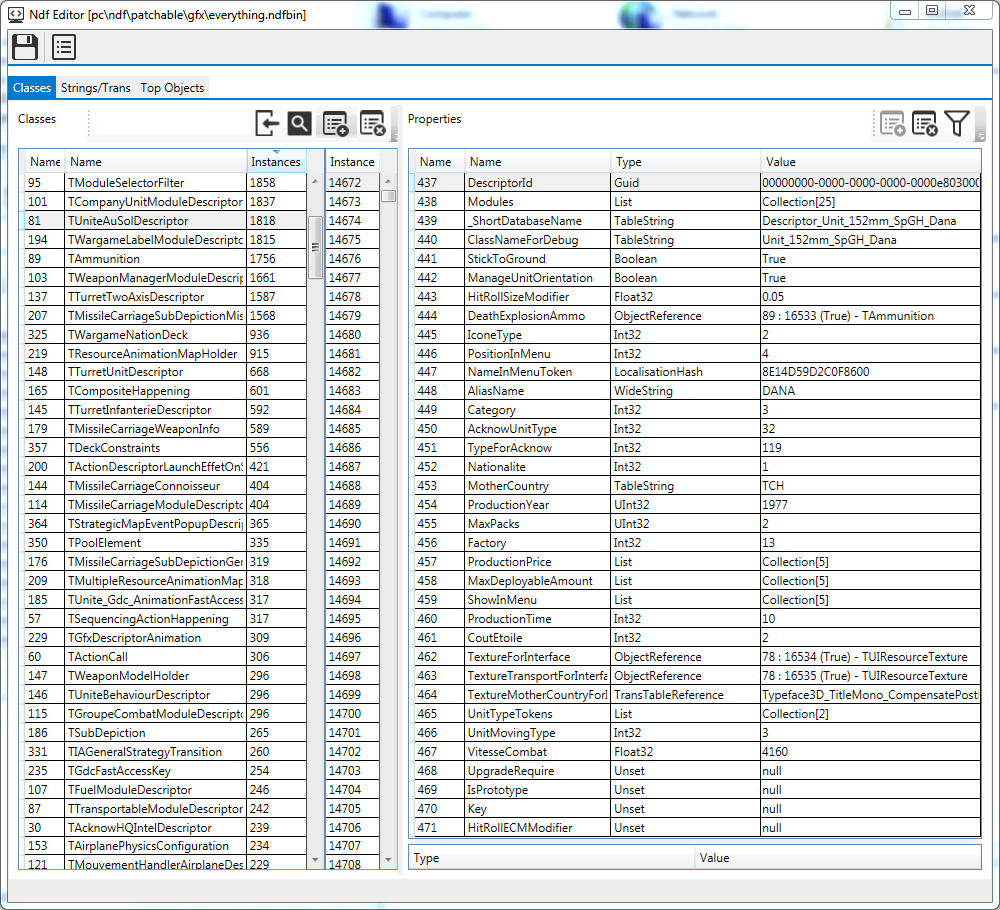
\includegraphics[width=0.8\textwidth]{screenshot_everything}


A sister table, TUniteDescriptor, describes both these units and additionally missiles, leading to a first, mildly amusing observation: missiles in the game are treated as their own units by the engine.

This table is our starting point.

Note that the first entry in this table is the 90-point Czech DANA artillery piece, which happens to, arbitrarily, have the lowest table ID in the game. This is followed by a Polish KUB-M anti-air unit, and then by a Russian Tunguska anit-air unit, as good a starting point as any other. 

\newpage

\section{TUniteAuSolDescriptor}

\subsection{DescriptorId}

This is a multi-part hex hash that is used internally by the engine. It is a unique key for the table. Don't touch it.

\subsection{\_ShortDatabaseName}

Prepended version of \_ClassNameForDebug.

\subsection{\_ClassNameForDebug}

An always-present non-localized unit name. Sometimes not entirely serious: for instance, Li Jian are given the moniker "Chinese Swords", while South Korean elite spec ops are "Black Berets". Not the name displayed in-game.

\subsection{StickToGround}

True if the unit is a ground unit, else null.

\subsection{ManageUnitOrientation}

Null for infantry units, True otherwise.

It is believed that this controls whether or not the unit can be given a position orientation command (Shift+Drag) in-game. 

\subsection{HitRollSizeModifier}

The effect that the size of the unit has on the chance-to-hit of other units firing at it. Larger-than-average units have a high HitRollSizeModifier, smaller-than-average ones have a low HitRollSizeModifier. This statistic is one of many calculations that factors into chance-to-hit.

The "Size" statistic in the armory screen is a direct translation of this variable. May be set to any float, but the values used in-game are:

\begin{center}
    \begin{tabular}{ | l | l | l | l | l |}
    \hline
	Value & Armory & Applies To & Example & Instances \\ \hline
	-0.2  &  Very Small & Scout helos & AH6C Little Bird  & 37\\
	-0.15 & Very Small & Infantry & Morskaya Pehota & 296 \\
	-0.1 & Very Small & Light helos & MI2URPG & 20 \\
	-0.05 & Small & Light vehicles & Scorpion Light Tank & 20\\
	null & Medium & Most things & BMP-1K & 958 \\
	0.05 & Big & Tanks, Heavy AA & M11P Abrams & 237\\
	0.1 & Very Big & Large helos & Mi-26 & 9\\	
    \hline
    \end{tabular}
\end{center}

\subsection{DeathExplosionAmmo}

A reference to a TAmmunition module which explodes in-place when this unit dies. This is a clever secondary use of TAmmunition, which is covered elsewhere in this guide.

At present time, units explode with one of just 11 animations. This includes null (e.g. no animation) which probably in error applies only to the Polish Star 266 supply truck.

\subsection{IconeType}

Unknown. Options are 1 (default), 2 (artillery and anti-ship missiles), and 3 (anti-air).

\subsection{PositionInMenu}

Does nothing.

\subsection{NameInMenuToken}

This localization hash controls the display name of the unit in the menu.

As previously mentioned, Wargame database files are backed up, with the structure and contents of each previous version of the game backed up in its own folder on disk. To get what this token corresponds to, we actually have to exit NDF\_Win.dat and load ZZ\_Win.dat instead (if this file is not present in your folder, check the immediately prior patch versions, one of them should have it). This file contains all of the text localization strings for the game. The \texttt{unites.dic} in particular contains all of the English-language menu texts, and if you for example look up our Dana's 8E14D59D2C0F8600 hash in this table you will find that it is, indeed, called the DANA in-game.

Thus you can change this yourself by editing this hash or by creating new ones and refering to them using the Modding Suite.

It needs to be noted that this piece of text corresponds to the name in the armory screen only. A second hash with the same name stored in the UnitType submodule, which we will get to later, controls the unit's name in-game.

\subsection{AliasName}

A better-formed name for the unit that appears, in most cases, to be a copy of NameInMenuToken. This variable does nothing in-game, however, is not editable, and is often (in 485 cases, as of writing) simply "null".

\subsection{Category}

Another categorization variable, filled in with a number between 1 and 6. What unit gets placed in what category does not appear to follow any logic, and this variable is safe to ignore.

\subsection{AcknowUnitType}

This variable categories units by type. The scattershot nature of the categorizations seems to imply that at one point the categorizations were of units of specific types, but balancing patches which moved these units around categories seem not to have included updates to this variable, introducing inaccuracies.

Given that fact, it is doubtful that this variable has effect on gameplay. See the "Factory" variable for a cleaner categorization variable.

\begin{center}
    \begin{tabular}{ | l | l |}
    \hline
	Value & Type\\ \hline
	15 & Israeli and Dutch (Paid DLC) Air Superiority Fighters.\\
	16 & Israeli and Dutch (Paid DLC) Multirole Planes.\\
	17 & Israeli and Dutch (Paid DLC) Ground-Attack Planes.\\
	18 & Israeli and Dutch (Paid DLC) SEAD Planes.\\
	22 & Tanks, and a few vehicles.\\
	23 & Missile platforms, mortars, most vehicles.\\
	24 & Most recon units.\\
	25 & Supply vehicles.\\
	26 & Command units.\\
	27 & Most planes and non-recon helicopters.\\
	28 & Flamethrower sappery.\\
	29 & Transport units, including commands based on them.\\
	30 & Missile-based anti-air, including anti-air infantry.\\
	31 & Gun-based anti-air.\\
	32 & Heavy artillery.\\
	33 & Most infantry.\\
	34 & Certain special forces infantry.\\
	35 & AsHMs, napalm launchers, and cluster artillery.\\
	36 & ATGM-carrying infantry and, weirdly, Mistrals.\\
	38 & Ships, including transport ships.\\
    \hline
    \end{tabular}
\end{center}

\subsection{TypeForAcknow}

Unknown.

\subsection{Nationalite}

NATO units are null, PACT units are 1.

\subsection{MotherCountry}

An abbreviation for the country of origin of this unit.

\begin{center}
    \begin{tabular}{ | l | l |}
    \hline
	Value & Nation\\ \hline
	US & United States\\
	UK & United Kingdom\\
	FR & France\\
	RFA & West Germany\\
	CAN & Canada\\
	SWE & Sweden\\
	NOR & Norway\\
	DAN & Denmark\\
	ANZ & ANZAC\\
	JAP & Japan\\
	ROK & South Korea\\
	ISR & Israel\\
	HOL & The Netherlands\\
	URSS & Soviet Union\\
	RDA & East Germany\\
	TCH & Czechoslavakia\\
	POL & Poland\\
	CHI & China\\
	NK & North Korea\\
    \hline
    \end{tabular}
\end{center}

These are French acronyms, hence why URSS is "backwards".

\subsection{ProductionYear}

The year that the unit was produced. Note that this variable only controls the text that displays on the unit card. Whether or not the unit is actually available in the unit-year categories for deck building (Cat A, Cat B, Cat C) is controlled by an element of the Filter field in the UnitType module.

The record for the oldest unit in the game goes to M-24, a ten-point Norwegian tank that is nothing less and nothing more than the same mainstay tank of World War II provenance. It has a build date of 1943.

Other ancient units are the Czech OT-810 halftrack (1945), Danish M6 Mosegris truck (1947), North Korean Su-76M tank destroyer (1948), and Soviet BTR-152E ZPTU-2 machine-gun truck (1950).

The newest units date to 1996, and include the K9 Thunder, AH-64 Escort, JAS-39 Gripen, AMOS, and Su-27PU.

\subsection{MaxPacks}

The number of cards of this unit which are available for deck-building. Ranges from 1 (542 instances) or 2 (995 instances, the most common) up to 9 (16 instances, for certain transports).

\subsection{Factory}

Armory tab. Values are:

\begin{center}
    \begin{tabular}{ | l | l | l |}
    \hline
	Value & Tab & Count\\ \hline
	3 & Logistics & 177\\
	6 & Infantry & 233\\
	7 & Planes & 214\\
	8 & Vehicles & 335\\
	9 & Tanks & 196\\
	10 & Recon & 197\\
	11 & Helicopters & 142\\
	12 & Ships & 65\\
	13 & Support & 259\\
    \hline
    \end{tabular}
\end{center}

\subsection{ProductionPrice}

The in-game production price. This value isn't provided straight, but is instead embedded into a Collection of five integer elements. This may be because production price was at one point experimentally dependent on the veterancy of the unit, but this mechanic is not used in-game. Instead, the first value in this list is the actual price, and the remainder are all placeholder values of 15.

\subsection{MaxDeployableAmount}

A Collection of integers. The amount of copies of this unit deployable at each veterancy level, per card. 0 for veterancies this unit is not available at. Ordered Rookie to Elite.

\subsection{ShowInMenu}

A Collection of booleans which is always set to True for true units and always set to False for missiles.

\subsection{ProductionTime}

How long it takes, between an air unit being clicked on or a squad of land units being places on the map, for the unit to appear where it's expected. Airplanes have a ProductionTime of null (instantaneous), most units have a ProductionTime of 10, and helicopters have a ProductionTime of 5. This value is in seconds.

\subsection{CoutEtiole}

Means "Price Star" in French. A quickly-dropped mechanic in the first iteration of the series, Wargame: European Escalation, was that unit cards for your deck, besides the basic ones, would cost an in-game currency known as "stars" to unlock. This variable used to control this cost, and continues to exist today as a holdover. Seems to always be set to 1, 2, or 3, and doesn't do anything.

\subsection{TextureForInterface}

A reference to the texture resource for this object's deck display.

\subsection{TextureTransportForInterface}

Transport units can appear in the armory screen as seperate units, but most of the time they are viewed during deck building "behind" the units they are carrying, in which case this texture reference is called up and placed. Is set to null for non-transport units.

\subsection{TextureMotherCountryForInterface}

Controls which flag gets displayed in the corner of the card display.

\subsection{UnitTypeTokens}

A list of LocalizationHash instances which control which deck type the unit falls into. Valid inputs are:

\begin{center}
    \begin{tabular}{ | l | l |}
    \hline
	Kind & Hash\\ \hline
	Mechanized & 8BD43C9757360E00\\
	Armored & 5C76718B57360E00\\
	Marine & 23B8605ED9380000\\
	Airborne & 0BB7685ED9380000\\
	Motorized & 5E767965E3000000\\
	Support & DAD77965E3000000\\
    \hline
    \end{tabular}
\end{center}

\subsection{UnitMovingType}

Flags the unit movement type. Values are:

\begin{center}
    \begin{tabular}{ | l | l | l |}
    \hline
	Value & Kind & Count\\ \hline
	1 & Foot & 296\\
	2 & Wheeled, Supply Truck, Land-Only & 36\\
	3 & Wheeled, Non-Supply Truck, Land-Only & 215\\
	5 & Tracked, Land-Only & 445\\
	6 & Planes, Helicopters & 448\\
	7 & Wheeled, Amphibious & 121\\
	8 & Tracked, Amphibious & 225\\
	9 & Ship & 32\\
    \hline
    \end{tabular}
\end{center}

A unit's track style controls how it moves, and this field contains some important information on this subject.

Units moving on foot (1) move at the same speed on land everywhere, can move on steep slopes, and cannot enter water. 

Wheeled units in general (2, 3, 7) move at 150 kph on roads, regardless of off-road speed (specified in MouvementManager), and move at 33\% of their off-road speed in forests. Amphibious wheeled units (7) can additionally enter water, moving at a globally-set 50\% of their off-road speed when doing so. I do not know what the difference between (2) and (3) is.

Tracked units in general (5, 8) move at 110 kph on roads, regardless of off-road speed (specified in MouvementManager), and move at 50\% of their off-road speed in forests. Amphibious tracked units (8) can additionally enter water, moving at a globally-set 50\% of their off-road speed when doing so.

It should be noted that while 150 kph and 110 kph are global values, they are not controlled globally. There is instead a multiplier in another submodule, MouvementDescriptor, called RoadSpeedBonus, which is always set to exactly what it has to be set to to make this fact true. Amphibiousness, by contrast, is universial: if the unit can tread water, it will do so at half of its off-road speed, and as no other variables control this behavior this happens without exceptions.

\subsection{VitesseCombat}

According to the name, the speed of the unit when it is in combat (e.g. whenever the unit can see enemy units). It is surprising that this is a top-level variable and unknown whether or not this variable has any effect. The input is an unsigned int; for information on what the unit of measurement is, refer elsewhere in this guide.

\subsection{UpgradeRequired}

Contains a reference to another TUniteAuSolDescriptor. When this unit is pulled up in the armory, assuming you did all of the other categorization placements right, this unit will display after the linked unit in the horizontal list. If this is set to null, the unit will appear either on its own line or as the first unit in the horizontal list, if another unit references it itself.

Five is the maximum value, as no more are allowed to stack in the armory; any number higher will move the unit to its own line. It's also notable that when transport units are linked via UpgradeRequired, if one unit is made available as a transport for a unit all of its children are, too (for example: enabling Mi-8T for Gornostrelki also enables Mi-8TVs).

\subsection{IsPrototype}

Whether or not the unit is a prototypal unit. Null if it isn't, True if it is. Affects deck-building, as prototypal units can't be used in global decks. 248 units in the game are considered prototypes, as of-writing, out of 1818 total, a little less than 14 percent of the total.

\subsection{Key}

Unknown. Almost always null.

\subsection{HitRollECMModifier}

The unit's ECM level. This only applies to planes and ships with higher than 0\% ECM; all other units (including planes without ECM) have this value set to null.

\subsection{Modules}

A list of submodules attached to this unit:


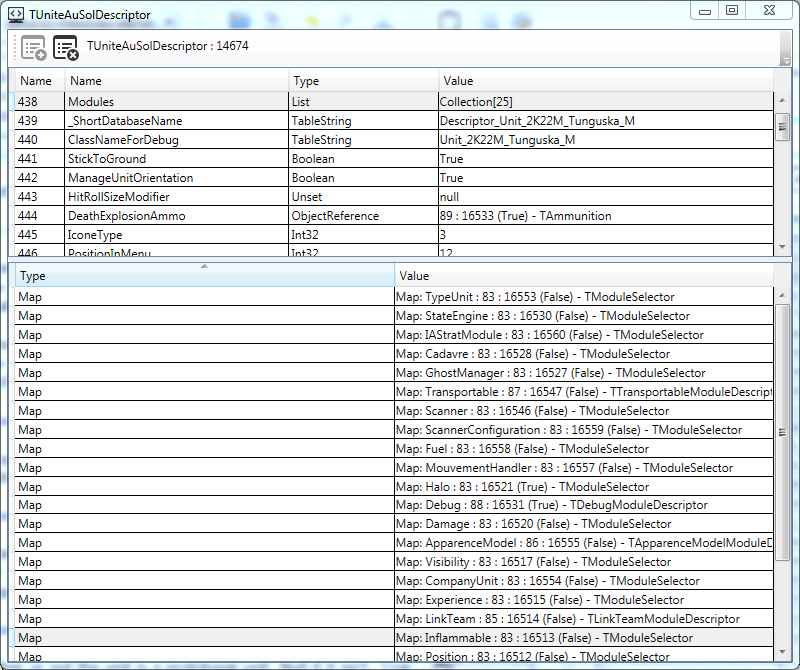
\includegraphics[width=0.8\textwidth]{screenshot_modules}

Each of these passes through a TModuleSelector to another table of some kind. We will now go through each of these in order of appearance.

\section{TTypeUnitModuleDescriptor}

\subsection{ControllerName}

Always TypeUnitController. Immutable.

\subsection{TypeUnitValue}

Unknown.

\subsection{TypeUnitHintToken}

Unknown.

\subsection{NameInMenuToken}

Just like its top-level NameInMenuToken, except that this copy of the hash controls what the unit's name is in-game, wheras the top-level one controls what it is in-menu. For more details see the UniteAuSol NameInMenuToken field.

\subsection{GenerateName}

Unknown. Always True.

\subsection{Filters}

This complex field is a Map containing four sets of things.

The first element is an in-game hover name which displays when a unit is hovered over by an enemy. An example value is "Anti-Air Vehicle".

The second element controls which of the year-based deck types the unit falls into (Cat A, Cat B, or Cat C). A dictionary for the values is:

\begin{center}
    \begin{tabular}{ | l | l | l |}
    \hline
	Value & Kind\\ \hline
41E22D4DD9380000 & 1980 and less\\
46E22D4DD9380000 & 1981 to 1985\\
81E22D4DD9380000 & 1986 and later\\
    \hline
    \end{tabular}
\end{center}

Note that it is this field, not the YearProduced top-level variable (which only controls an element of the card display), which controls which year-limited deck categories the unit is available in.

The third element is a set of the deck types that the unit appears in. But wait, you may ask, doesn't the top-level UnitTypeTokens already do that? It turns out that to make things work you have to properly set both that value and this one. Again, here's a list of valid hashes:

\begin{center}
    \begin{tabular}{ | l | l |}
    \hline
	Kind & Hash\\ \hline
	Mechanized & 8BD43C9757360E00\\
	Armored & 5C76718B57360E00\\
	Marine & 23B8605ED9380000\\
	Airborne & 0BB7685ED9380000\\
	Motorized & 5E767965E3000000\\
	Support & DAD77965E3000000\\
    \hline
    \end{tabular}
\end{center}

The fourth element is a set of hashes for miscellaneous filters that the unit falls under in the armoy. So for example if you want a unit to fall the "Cavalry Tank" filter there, you would need to set the appropriate hash here. The values for these hashes in particular are located in the interface\_ingame.dic file inside ZZ\_Win.dat.

\subsection{MotherCountry}

A copy of the top-level attribute.

\subsection{UnitInfoJaugeType}

Unknown.

\subsection{Training}

If this unit is an infantry unit, this is set to a hash pointing to its training level (otherwise null):

\begin{center}
    \begin{tabular}{ | l | l | l |}
    \hline
	Kind & Hash & Count\\ \hline
	Elite & 8F37594F19619C07 & 45\\
	Shock & 5593495D19619C07 & 66\\
	Regular & D6173D5C19619C07 & 164\\
	Militia & DE644D5719619C07 & 15\\
    \hline
    \end{tabular}
\end{center}

\subsection{CIWS}

The CIWS statistic, as displayed in the armory, carried by a naval unit. Set to null for non-naval units and for naval units without CIWS. This is a localization hash; to set it to a particular value, use one of the following:

\begin{center}
    \begin{tabular}{ | l | l | l |}
    \hline
	Kind & Hash & Count\\ \hline
	Exceptional & 4F233E0000000000 & 1\\
	Very Good & 4E96452000000000 & 3\\
	Good & 4E96450000000000 & 4\\
	Medium & D672711906000000 & 6\\
	Bad & CEC2000000000000 & 15\\
	None & null & 1786\\
    \hline
    \end{tabular}
\end{center}

Changing this value does NOT change a ship's CIWS, it only changes the quality of CIWS reported on the card in-game. In other words, this only controls a text display element.

\subsection{Sailing}

The ship's sailing type. This is similarly a LocalizationHash controlling a text display, not the real value (which is in MouvementControl). Values are:

\begin{center}
    \begin{tabular}{ | l | l |}
    \hline
	Kind & Hash\\ \hline
	Deep Sea & CBD32D65B4780000\\
	Coastal & CBD33165B4780000\\
	Riverine & CBD33565B4780000\\
	None & null\\
    \hline
    \end{tabular}
\end{center}

\section{TDebugModuleDescriptor}

There is nothing interesting here.

\section{TStateEngineModuleDescriptor}

There is nothing interesting here.

\section{TFlagsModuleDesciptor}

Uknown.

\section{TCriticalEffectModuleDesciptor}

A reference to one of a small number of tables which control the critical effects a unit may be subjected to that occur due to fire from enemy units (critical effects affecting movement are in a different module, Mouvement). We will omit further details, as the resultant tables are various, singular, and pretty easy to parse.

\section{TTargetCoordinatorModuleDescriptor}

There is nothing interesting here.

\section{TPositionModuleDescriptor}

\subsection{ControllerName}

Not interesting.

\subsection{InGeoDb}

Unknown.

\subsection{ClampInWorld}

Unknown.

\subsection{GfxDescriptorPorteur}

Links to a module containing information of interest to the physics engine, which shouldn't be messed with.

\subsection{Radius}

Unknown.

\subsection{AddToHexagonMap}

Unknown.

\subsection{PorteurMustBeVisible}

Unknown.

\subsection{RelativeScanningPosition}

Unknown.

\subsection{CameraFollower}

Links to a TGfxDescriptorCameraFollower object that sets variables for the camera, meant for focus-watching a plane, land unit, ship, or helicopter.

\subsection{MustAllowZoneIndice}

Unknown.

\subsection{LowAltitudeFlyingAltitude}

If the unit is a helo, the altitude that the helo flies at by default.

\subsection{NearGroundFlyingAltitude}

If the unit is a helo, the altitude the helo goes to when told to descend (which helps with stealth, but is barely ever used anymore).

\subsection{ClampOutMap}

Unknown, always null.

\subsection{HasNearlyNullBBox}

Unknown, always null.

\subsection{\_ShortDatabaseName}

Useless, always null.

\section{TInfammableModuleDescriptor}

There is nothing interesting here.

\section{TLinkTeamModuleDescriptor}

There is nothing interesting here.

\section{TModernWarfareExperienceManagerDescriptor}

\subsection{ControllerName}

Disinteresting.

\subsection{CanWinExperience}

There are only two possible table references: one with CanWinExperience set to null, which is applied to supply units and units without weapons, and one with CanWinExperience set to True, for everything else.

\subsection{ExperienceGainBySecond}

Always set to 0.1.

\subsection{KillExperienceBonus}

Always set to 2.5

\section{TIAStratModule}

This module contains a few hard-coded numerical references which are used for internal AI orchestration.

\section{TModernWarfareCadavreModuleDescriptor}

This module is buried in the logic section of the CadavreController top-level module object. It contains a number of interesting variables, all controlling what happens when a unit dies: how long it sticks around afterwards, how quickly it fades, whether or not it exploded on death (if it does, it uses the DeathExplosionAmmo top-level object), and a bunch of flags:

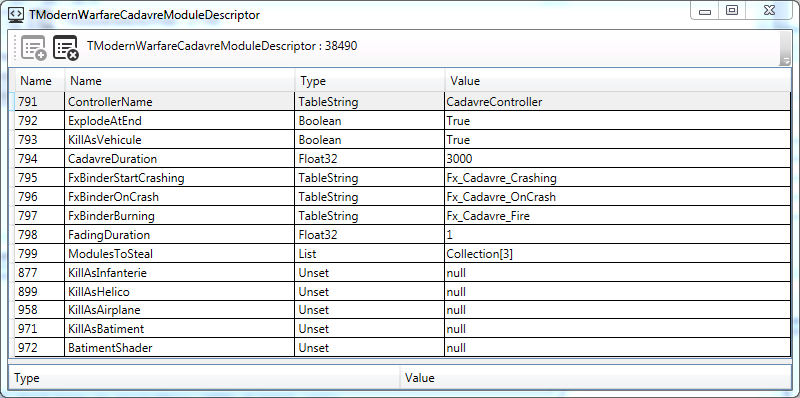
\includegraphics[width=0.8\textwidth]{screenshot_cadavre}

We will omit examining it in detail.

\section{TTurretSkeletonModuleDescriptor}

Contains a pointer to the unit's primary mesh.

\section{TMissileCarriageModuleDescriptor}

Contains pointers to art resources constituting missile carriages, which control all of the art involved in units having and then not having certain visible weapon elements on-body. So for example, a F-15D Eagle with its bombs would look different from an F-15D Eagle without its bombs, obviously. That's controlled here.

We will omit further details, except to say that the difficulties of working with this module make modding planes and helicopters (some of which have this module, some of which haven't) challenging.

\section{TCommandManagerModuleDescriptor}

When this module is set up properly, the unit is treated as a command unit in-game.

\section{TGhostManagerModuleDescriptor}

This module controls things related to what happens when a unit is spotted, but not identified: what you see when something is shaded in black. 

\section{TScannerModuleDescriptor}

This module is only present if the unit has special vision privileges. It contains a TModernWarfareVisibilityRollRule as a subtable, which in turn contains TModernWarfareVisibilityRollRuleDescriptor and TModernWarfareDistanceMultiplierRollRuleDescriptor dependencies.

A relatively small number of tables of the latter two types ultimately control large swatches of unit vision ranges, so you might find that e.g. tweaking one Very Good recon unit's table's vision range up will turn up vision for ALL Very Good recon units, and other similar shenanigans.

Types of vision controlled by this module are Air, Sea, and Land.

This module only contains multipliers. Base vision values are set by the module below.

\section{TScannerConfigurationDescriptor}

This module, if present, controls the base vision values for units granted above-normal vision. All of the base values come from here, but interact with values in TScannerModuleDescriptor above. If one of these two modules is present, both are, as they are dependent on one another.

\subsection{ControllerName}

Always ScannerConfigurationController. Immutable.

\subsection{UnitType}

A reference to the domain of the unit in question itself. UnitType 1 refers to ground, UnitType 4 refers to planes, and UnitType 6 refers to ships.

\subsection{DetectionTBA}

Maximum range at which you can see an unidentified helicopter.

\subsection{PorteeVision}

Maximum range at which you can see an unidentified ground unit.

\subsection{OpticalStrength}

Optical strength against ground units, used to determine whether a unit can see enemy units in cover.

\subsection{OpticalStrengthAltitude}

Optical strength against aircraft (including helicopters).

\subsection{SpecializedOpticalStrengths}

This is a Collection of float pair mapping; each of the maps binds a UnitType and then the range at which they can be detected. UnitType 4 refers to planes, while UnitType 6 refers to ships, and UnitType 1 refers to Land. The value Optican strengths against 

\subsection{SpecializedDetections}

Maximum range at which you can see an unidentified unit. This is a Collection of float pair mapping; each of the maps binds a UnitType and then the range at which they can be detected. UnitType 4 refers to planes, while UnitType 6 refers to ships, and UnitType 1 refers to Land.

\subsection{PorteVisionTBA}

Maximum spotting range for helicopters. This attribute is only populated for helicopters, in which case it controls helicopter-to-helicopter sighting. It is otherwise null.

\subsection{OpticanStrengthAntiradar}

Maximum anti-radar spotting range. Only populated for anti-radar units; null otherwise.

\subsection{\_ShortDatabaseName}

Same as the top-level parameter, but this seems to always be null.

\section{TFuelModuleDescriptor}

\subsection{ControllerName}

Uninteresting.

\subsection{FuelCapacity}

The number of units of fuel that this unit carries. While actual autonomy is a function of FuelMoveDuration, this variable controls fuel efficiency with respect to that, and, therefore, how expensive it is to refuel this unit. This variable ranges between 45 (the L3304, a Sewidish recon jeep) and 6500 liters (Su-24, MiG-31, MiG-25, F-15, F-14, and F-111 series planes).

\subsection{FuelMoveDuration}

Autonomy in seconds. Appears to be the same as the T.O.T statistic displayed in the Armory. Ranges between 60 (MiG-17, F-5, and other cheap planes) and 2000 (CH-46 Phrog, CH-47 Chinook, and MH-53 Pave Low variants).

\section{TMouvementHandlerLandVehicleDescriptor}

This module is present in the TMouvementDescriptor slot if and only if the unit is a land unit, or, interestingly enough, a ship.

\subsection{ControllerName}

Uninteresting.

\subsection{Maxspeed}

The unit's max speed, in engine distance units (see the next major section for unit explanations).

\subsection{UnitMovingType}

The same as that set in TUnitMouvementDescriptor.

\subsection{SpeedBonusOnRoad}

A multiplier on the unit's base speed. Always set to whatever it needs to be set to to give the unit 110kph tracked speed or 150kph wheeled speed, meaning that these are constants but must be set on the local level! If this unit is a ship, this value is instead set to null.

\subsection{TempsDemiTour}

The amount of time, in seconds, it takes for a unit to make a half-turn (the translation is literal). If you tell a land unit to move in a direction directly opposite to its current orientation, it will do a reverse-accelerate V-turn to the side, and this variable controls how long this takes. Ships will execute their turn completely in place (unrealistically but necessarily, given how the game works).

Presumably this value also controls how long it takes to make turns that are less than 180 degrees, but still significant. The cutoff value at which a unit starts to make a reverse turn, instead of just turning in place, is unknown.

\begin{center}
    \begin{tabular}{ | l | l | l |}
    \hline
	Value & Units & Count\\ \hline
	0.1 & Infantry & 296\\
	2.0 & Jeeps & 236\\
	3.0 & Light vehicles & 404\\
	4.0 & Trucks, heavy vehicles, light tanks & 167\\
	5.0 & Most tanks & 366\\
	6.0 & Artillery, MLRS, Challenger 1 series tanks & 60\\
	7.0 & Some MLRS, some tanks (Centurions, Chieftains) & 44\\
	10.0 & Light ships & 8\\
	15.0 & Heavy ships & 5\\
	20.0 & Fleet ships (Sovremenniy, Udaloy II, Kongo) & 3\\
    \hline
    \end{tabular}
\end{center}

\subsection{MaxAcceleration}

The acceleration the unit applies when it is speeding up.

\begin{center}
    \begin{tabular}{ | l | l | l |}
    \hline
	Value & Units & Count\\ \hline
	4030 & Infantry & 296\\
	2080 & Jeeps & 100\\
	1950 & Light vehicles & 131\\
	1560 & T-64BM, T-72S Series, T-72M2 Moderna & 7\\
	1300 & Most tanks and vehicles & 443\\
	1040 & Centurion series tanks, PTZ-59, ZTZ-59-II & 15\\
    \hline
    \end{tabular}
\end{center}

\subsection{MaxDeceleration}

How hard to breaks hit. Always 4030 for infantry and 2600 for everything else.

\subsection{VehicleSubType}

1 for lightly armored units, 2 for infantry, 3 for other lightly armored stuff, and 4 for boats. More often then not, however, this variable is set to null, and so may be safely ignored.

\subsection{CriticalEffectModule}

A module pointer whose contents is a TCriticalEffectModuleDescriptor describing what happens when this units is hit with a critical. Unfortunately it ultimately points to hashes, not to any descriptions of the effects of the criticals themselves...

\subsection{TerrainsToIgnoreMask}

This is set to certain magic values for ship units which are allowed and not allowed to enter different water depths: 16 if it can enter all waters, 24 if it's a coaster, and 26 if it's a bluewater ship.

Otherwise null.

\section{TMouvementHandlerHelicopterDescriptor}

This module is present in the TMouvementDescriptor slot if and only if the unit is a helicopter.

\subsection{ControllerName}

Uninteresting.

\subsection{Maxspeed}

The unit's max speed, in engine distance units (the meaning of which is covered elsewhere).

\subsection{MaxAcceleration}

The acceleration the unit applies when it is speeding up.

\begin{center}
    \begin{tabular}{ | l | l | l |}
    \hline
	Value & Examples & Count\\ \hline
	2080 & AH-1 Cobra, Z-9, Gazelle & 93\\
	1560 & AH-64, Tigre, Mi-28 & 17\\
	1040 & Mi-8, UH-1H Huey, Mi-24, CH-47 Chinook & 109\\
    \hline
    \end{tabular}
\end{center}

\subsection{MaxDeceleration}

How hard the breaks hit. The values are always the same as those above (e.g. helicopters always decelerate and accelerate at the same rate).

\subsection{UnitMovingType}

The same as that set in TUnitMouvementDescriptor. Here this will always be 6, for air.

\subsection{CyclicManoeuvrability}

Controls movement in some way, though in what way is uncertain. Higher is better.

\begin{center}
    \begin{tabular}{ | l | l | l |}
    \hline
	Value & Examples & Count\\ \hline
	40 & CH-47C Chinook, Mi-6, Mi-26 & 22\\
	60 & Mi-4, Mi-8, Mi-17 & 31\\
	80 & Mi-24, Ka-29TB, UH-1H Huey & 46\\
	90 & PUMA 330, Z-9 & 11\\
	100 & Mi-2, AH-64, Ka-52 & 34\\
	110 & Z-9, Lynx, Alouette & 22\\
	130 & Gazelle, AH-1 Cobra, Bo-105 & 53\\
    \hline
    \end{tabular}
\end{center}

\subsection{GFactorLimit}

Controls movement in some way, though in what way is uncertain.

\begin{center}
    \begin{tabular}{ | l | l | l |}
    \hline
	Value & Examples & Count\\ \hline
	1.8 & CH-47C Chinook, Mi-6, Mi-26 & 53\\
	2.2 & UH-1H Huey, Bell 412 & 25\\
	2.5 & Mi-2, Mi-24, Lynx & 70\\
	3.0 & AH-64, Ka-52, Tigre & 15\\
	3.5 & Gazelle, AH-1 Cobra, Bo-105 & 56\\
    \hline
    \end{tabular}
\end{center}

\subsection{LateralSpeed}

Controls movement in some way, though in what way is uncertain. Is always set to 2600.

\subsection{Mass}

Controls movement in some way, though in what way is uncertain.

Values used in-game are 50000.0, 22000.0, 12000.0, 11000.0, 10000.0, 8500.0, 8000.0, 7000.0, 5300.0, 4300.0, 4100.0, 3700.0, 3000.0, 2500.0, or 1800.0.

\subsection{MaxInclination}

Controls movement in some way, though in what way is uncertain.

\begin{center}
    \begin{tabular}{ | l | l | l |}
    \hline
	Value & Examples & Count\\ \hline
	89 & Mi-2, Mi-24, Lynx AH.7 & 154\\
	80 & PUMA, Z-9 & 11\\
	75 & PUMA 330B Command & 1\\
	60 & Mi-8, CH-47 Chinook & 53\\
    \hline
    \end{tabular}
\end{center}

\subsection{RotorArea}

Controls movement in some way, though in what way is uncertain. Ranges between 80 and 800.

\subsection{TorqueManoeuvrability}

Controls movement in some way, though in what way is uncertain. Ranges between 30 and 120.

\subsection{UpwardsSpeed}

Controls movement in some way, though in what way is uncertain. Ranges between 1300 and 3900.

\subsection{CriticalEffectsModule}

A module pointer whose contents is a TCriticalEffectModuleDescriptor describing what happens when this units is hit with a critical. Unfortunately it ultimately points to hashes, not to any descriptions of the effects of the criticals themselves...

\subsection{TempsDemiTour}

The amount of time, in seconds, it takes for a unit to make a half-turn (the translation is literal). For helicopters this requires a dive to the left. For helicopters this variable is always set to 2.

\section{TMouvementHandlerAirplaneDescriptor}

This module is present in the TMouvementDescriptor slot if and only if the unit is a plane.

\subsection{Maxspeed}

Maximum speed this unit can go at. Since airplanes fly at a constant speed, this is also the only speed.

\subsection{UnitMovingType}

Always 6, for air.

\subsection{FlyingAltitude}

The height the plane prefers to fly at. Notably, all planes spawn at the same height then ascend or descend to their prefered height.

\begin{center}
    \begin{tabular}{ | l | l | l |}
    \hline
	Value & Examples & Count\\ \hline
	78000 & F-117 Nighthawk, B-5, MiG-31M, F-14 Tomcat & 7\\
	65000 & EF-111A Raven, Eurofighter Typhoon & 78\\
	52000 & A-5, A-4K Kahu, CF-18 Hornet & 61\\
	39000 & F-111C, A-6A Intruder, Alpha Jet A & 26\\
	26000 & A-10 Thunderbolt II, F-111G. CF-104 & 51\\
    \hline
    \end{tabular}
\end{center}


\subsection{MinimalAltitude}

Below which the plane will not dip. Will cause it to break off from certain attacks at certain heights.

\begin{center}
    \begin{tabular}{ | l | l | l |}
    \hline
	Value & Examples & Count\\ \hline
	15600 &  F-117 Nighthawk, B-5, MiG-31M, F-14 Tomcat & 7\\
	13000 & EF-111A Raven, Eurofighter Typhoon & 78\\
	10400 & A-5, A-4K Kahu, CF-18 Hornet & 67\\
	7800 & F-111C, A-6A Intruder, Alpha Jet A & 26\\
	5200 & A-10 Thunderbolt II, F-111G. CF-104 & 49\\
	2600 & J-35D Draken, J-35F Draken & 2\\
    \hline
    \end{tabular}
\end{center}

\subsection{PhysicsConfiguration}

A reference to a TAirplanePhysicsConfiguration module, which controls the plane's various movement parameters.

\subsection{CriticalEffectsModule}

A module pointer whose contents is a TCriticalEffectModuleDescriptor describing what happens when this units is hit with a critical. Unfortunately it ultimately points to hashes, not to any descriptions of the effects of the criticals themselves...

\subsection{GunMuzzleSpeed}

Unknown. Always 300000.

\subsection{LandingGearOutPhysicalPropertyName}

Unknown. Always "InShowRoom".

\subsection{LandingGearSubDescriptionName}

Unknown. Always "Landing Gear".

\subsection{FrontLandingGearMeshNodeName}

Unknown. Always "Train\_Avant".

\subsection{BackLandingGearMeshNodeName}

Unknown. Always "Train\_Arriere".

\section{THaloModuleDescriptor}

Does a bunch of things which control the circle that gets drawn when a unit is selected.

\section{TGroupeCombatModuleDescriptor}

This module, which is only attached to infantry units. This table has a submodule, TUniteBehaviorDescriptor, which has a large number of variables controlling the unique aspects of infantry combat stats in the game.

Amongst the various TUniteBehaviorDescriptor tables, all of the variables contained therein are the same (making them globals, essentially) except for two: NbSoldatInGroupeCombat, which controls the number of men to the squad, and AnimationFastAccessor, whose purpose is unknown.

\section{TTransportableModuleDescriptor}

This module, which is only attached to infantry units, controls what transports are available to an infantry unit.

\subsection{ControllerName}

Not interesting.

\subsection{Categories}

Always a list with two elements: "infantrie" and "barge".

\subsection{SuppressDamageRatioIfTransporterKilled}

This float controls what percentage of the unit's total suppression cealing (which is 800 for all units) the unit will take in suppression damage if it is on a transport, the transport is destroyed, and the unit survives.

As such it contains direct references to other transporter units' TUniteAuSolDescriptor instances.

\subsection{TransportListAvailableForSpawn}

This contains a Collection of references to one or more transporter units' TUniteAuSolDescriptor instances. Those units become available to this unit as an on-card transport.

Note that, due to the previously described mechanics of the UpgradeRequired top-level variable, a reference in this table to a transporter unit with an upgrade path will cause all of those other units to also become available. So the exactly list of transporters for this unit may be longer than it appears to be from this list alone!

\subsection{TransportedTexture}

Unknown. Transported units have no texture, no?

\section{TModuleModernWarfareSupplyDescriptor}

\subsection{ControllerName}

Uninteresting.

\subsection{SupplyCapacity}

Units of supply (liters) this unit carries. Ranges between 15000 and 500.

\subsection{DeploymentDuration}

How long after a unit has stopped before it begins to provide supply, in seconds. Always 0.2 seconds currently, except for FOBs, which have this value set to null.

\subsection{WithdrawalDuration}

How long after a unit is ordered to start moving before it stops providing supplies and starts moving. Currently always 0.2 seconds currently, except for FOBs, which have this value set to null.

\subsection{SupplyPriority}

It is possible for supply units to supply other supply units; for example a common tactic is to shorten the supply chain trip length by buying a Mi-26, dropping it halfway between the FOB and the battlefield, and running ammo trucks between the helo and the front line. The lower this number the lower in this stack this unit is, and the greater the number of other supply units this supply unit could itself draw from. Generally 1-to-1 with total supply onboard: the bigger the capacity, the lower the SupplyPriority.

Ranges between 10 and 34.

\subsection{SupplyDescriptor}

Links to another module, an instance of TModernWarfareSupplyDescriptor, which contains the variables used for calculating supply cost and supply per second. There are only two instances of TModernWarfareSupplyDescriptor, one for FOBs and one for all other supply units. The latter includes the following essentially-globals:

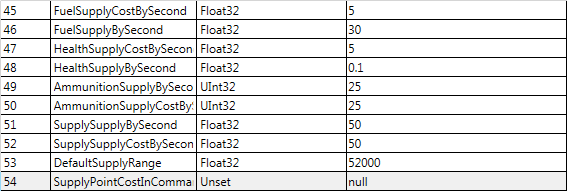
\includegraphics[width=0.8\textwidth]{screenshot_supply}

The former:

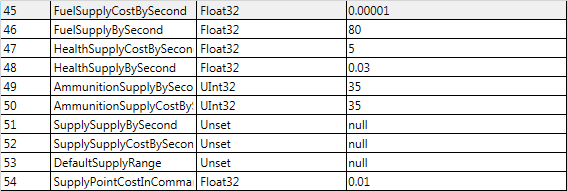
\includegraphics[width=0.8\textwidth]{screenshot_supply_fob}

\section{TWeaponManagerModuleDescriptor}

This is one of the two most interesting modules overall, and easily the most complicated one. This module controls everything that there is to know about a unit's weaponry, and to understand its logical structure is to understand how weapons in this game work.

Each TWeaponManagerModuleDescriptor contains a Collection known as a TurretDescriptorList whose items are individual TTurretTwoAxisDescriptor, TTurretUnitDescriptor, TTurretInfanterieDescriptor, or TTurretBombardierDescriptor modules.

These names pretty descriptively describe which particular module type corresponds with which weapon domain, and each one describes the weaponry and behavior of a turret of some kind on the unit. Each individual weapon, the things you actually see on the unit card, is in turn one of the TMountedWeaponDescriptor modules in the list of them stored in the MountedWeaponDescriptorList attribute of TTurret\textless *\textgreater Descriptor.

Each of these in turn contains a reference to a single TAmmunition object, which describes everything about the damage output of the weapon itself, as opposed to the way it's mounted.

And TAmmunition can itself contain references to another object! That object will be a TUniteDescriptor instance describing what the missile or round looks like and acts like while it's in flight.

This a very dense structure, and it takes some play and mucking about to make sense of it at all.

\subsection{ControllerName}

Not interesting.

\subsection{\_ShortDatabaseName}

Will be "WeaponDescriptor\_" followed by the unit's debug name. Not very interesting.

\subsection{HasMainSalvo}

You may notice that almost all air unit will automatically "Evac Winchester" when a certain condition or set of condition is met. For air-to-ground units, this will occur whenever the unit has dropped its payload; for air-to-air units, it will occur when it has run out of missiles. There are a few corner cases, like the A-10 Thunderbolt, whose cannon is considered an important enough arnament that it doesn't just evac when it runs out of Mavericks; but it will if it runs out of both missiles and gun rounds (somehow).

This flag indicates whether or not the unit has such a salvo. It is set to true if it does, and set to null if it doesn't. All non-plane units have this set to null.

\subsection{SalvoIsMainSalvo}

This is always a collection of four booleans. Note that it does nothing if HasMainSalvo is null, but is not itself null in that case. We therefore restrict our attention to the case of planes.

The first element controls whether or not the weapon tagged to the first salvo index is considered the main weapon. For planes, the first salvo index will always be the gun, so the boolean in this index will control whether or not the plane's gun is considered primary.

Again in the case of planes, the second element is never tagged to anything, so this is always False.

The third element is whatever is tagged to the second salvo index, and the fourth element is whatever is tagged to the third salvo index.

What do I mean by "tagged to the nth salvo index"? That's convered by the next variable.

\subsection{Salves}

Salves is a variable containing the number of salvos of a weapon available to a unit.

For example, if a unit has a salvo size (set by NbTirParSalve three levels of heirarchy below, in TAmmunition) of 24 shots per salvo, and the corresponding entry in Salves gives is a value of 2, then the unit will have two salvos of 24 shots each. For an explanation of what a salvo is, refer to the TAmmunition documentation.

Weapons are not listed in Salves in the order that they appear on the unit card. The order that they do appear in somewhat defines explanation. Salves always has 29 values in it, corresponding with a theoretical 29 weapons; in cases in which there is no weapon corresponding with that slot, the value is filled in as a -1.

Which weapon corresponds to which index in this list is controlled by SalvoStockIndex, two levels of heirarchy down in TMountedWeaponDescriptor.

\subsection{TurretDescriptorList}

This is the next level of heirarchy down. Keep reading the section immediately below to study what's found here.

\section{TurretDescriptorList : TTurret\textless *\textgreater Descriptor}

As previously described, each TWeaponManagerModuleDescriptor contains a Collection known as a TurretDescriptorList whose items are individual TTurretTwoAxisDescriptor, TTurretUnitDescriptor, TTurretInfanterieDescriptor, or TTurretBombardierDescriptor modules. In this section we will describe the components of these modules.

\subsection{NbFx}

Something related to the physics engine.

\subsection{Tag}

The tag will a string of the form "tourelle1", "tourelle2", etcetera. This explicitly states the position of the turret in question in the list of turrets. Turrets are always tagged in the same order that they appear in thee TurretDescriptorList. This property will not appear for TTurretIfanterieDescriptor modules.

\subsection{TagIndex}

An even more literal intepretation of the above: will be one of 1, 2, 3, and so on. This property will not appear for TTurretIfanterieDescriptor modules.

\subsection{VitesseRotation}

Traverse speed of the turret, presumably in radians per second. This only appears if the turret in question is capable of traversal, so it is limited to TTurretTwoAxisDescriptor instances. Ranges between 1300 (I-Hawk family) and 36400 (the Pegasus).

\subsection{AngleRotationBase}

The angle that the turret has with the hull when idle, in radians. This property is unique to TTurretTwoAxisDescriptor instances.

\subsection{AngleRotationMax}

Is the maximum angle that the turret can traverse. If you were to set this value to ~6.28, approximately 360 degrees, the turret traversal is 360 all around. This property will not appear for TTurretIfanterieDescriptor modules.

\subsection{AngleRotationMaxPitch}

Maximum turret elevation. This property will not appear for TTurretIfanterieDescriptor modules.

\subsection{AngleRotationMinPitch}

Minimum turret depression. This property will not appear for TTurretIfanterieDescriptor modules.

\subsection{AngleRotationBasePitch}

Resting turret depression. This property is unique to TTurretTwoAxisDescriptor instances.

\subsection{UnitIdleManagerDescriptor}

If this turret does something when the unit is idle (tank cannons for example will return their resting position), then this action is controlled by a module reference in this field. We will omit exploring that in detail. Only TTurretTwoAxisDescriptor instances have this attribute. This property is unique to TTurretTwoAxisDescriptor instances.

\subsection{TargetPositionPhysicalPropertyName}

Unknown.

\subsection{FlyingTimeAndHitPhysicalPropertyName}

Unknown.

\subsection{OwnerTurnHisChassisVerticallyToAttack}

This variable controls whether or not the unit automatically turns towards its target vertically. Whether or not the unit turns its chassis horizontally is controlled elsewhere, by the AutoRotation parameter in the UnitMouvement module field. This field is null for all land units, which obviously can't turn vertically. It is set to true for fixed-axis weapons, like helicopter or plane unguided rocket pods for example.

This property will not appear for TTurretIfanterieDescriptor modules.

\subsection{MountedWeaponDescriptorList}

This property contains a list of references to the TMountedWeaponDescriptor elements mounted on this turret. This is the next level of heirarchy down, and is considered in the next section.

\section{TTurret\textless *\textgreater Descriptor : TMountedWeaponDescriptor}

Each individual weapon, the things you actually see on the unit card, is one of the TMountedWeaponDescriptor modules in the list of them stored in the MountedWeaponDescriptorList attribute of TTurret\textless *\textgreater Descriptor.

Note that within the game files a unit can have more weapons than appears on its cards. This is true in part because weapons which deal both AP and HE or which can fire smoke have seperate weapons for each of these "features", and in part because ships have far more weapons than is listed on their card. The recordholder in this regard is, suprisingly, the Najin, which packs 11 weapons onboard. Way more than the 3 you see on the card!

\subsection{SalvoStockIndex}

Which position in the Salves list two levels of heirarchy up, in the base TWeaponManagerModuleDescriptor, the current weapon takes it salvo count from. A small but important technical rub: if this value is set to null, then it is equivalent to the first value in the Salve list (the zeroth index).

\subsection{SalvoStock\_ForInterface}

This variable controls which position, amongst the weapons displayed on the unit card, the weapon in question occupies. Some weapons are defined twice, once for HE and once for AP, and they may have the same SalvoStock\_ForInterface value, in which case the two weapons will "stack" in the card display (resulting in a weapon with both HE and AP power, as with all tank cannons for example).

\subsection{EffectTag}

Unknown.

\subsection{TirContinu}

Unknown.

\subsection{TirEnMouvement}

Whether or not this weapon can be fired on the move. Null if no (grants the [STAT] tag), True is yes (in which case if additionally MissileDescriptor is populated and IsFireAndForget is set to True, then this weapon is [F\&F]; otherwise if MissileDescriptor is populated and IsFireAndForget is False, this weapon is [SA]; if MissileDescriptor is null this weapon recieves no additional tag). Note that the actual moving accuracy is set within the HitRollRule inside of TAmmunition, two levels of heirarchy deeper.

\subsection{AnimateOnlyOneSoldier}

This variable is set to null if the unit in question is not an infantry unit. If it is, and the weapon in question is a squad weapon limited only to the first man in the squad, then this value is set to True.

\subsection{Ammunition}

The next level of heirarchy. Keep reading...

\section{Ammunition : TAmmunition}

Describes everything about the damage output of the weapon itself, as opposed to the way it's mounted.

\subsection{DescriptorId}

An internal database hash. Don't touch this.

\subsection{Name}

An LocalizationHash which points at a ZZ\_Win.dat file (whicn one?)  to find a name for the cannon as displayed on the unit card. For example, the main cannon of an M1A1 is named M256.

\subsection{TypeName}

Unknown.

\subsection{TypeArme}

This LocalizationHash points at a ZZ\_Win.dat file to find the weapon type. Here are the known hash values:

\begin{center}
    \begin{tabular}{ | l | l | l |}
    \hline
	Hash & Kind & Count\\ \hline
	B31E95B36B5E0000 & Main Gun & 639\\
	D175010000000000 & MMG & 569\\
	F46CA274AE2F0000 & Autocannon & 436\\
	5C99C7BA89E30B00 & Assault Rifle & 342\\
	57E42D0000000000 & ATGM & 272\\
	D7B2000000000000 & Air-to-Air Missile & 187\\
	E162010000000000 & Light Anti-Tank Weapon & 185\\
	6ABCBA1C00000000 & Battle Rifle & 160\\
	D7D2010000000000 & SAM & 149\\
	B7FAE72E4F4B0000 & Howitzer & 130\\
	E1D2010000000000 & CQC LMG & 97\\
	295D975EC5010000 & Rocket Pods & 97\\
	D1D5010000000000 & SMG & 84\\
	B799DFF405000000 & Mortar & 74\\
	D125010000000000 & HMG & 72\\
	D165010000000000 & LMG & 66\\
	74AE2FE5ECF21E00 & Twin Autocannon & 65\\
	57D7010000000000 & AShM & 61\\
	ECECC6B919010000 & Gatling Gun & 56\\
	5C19BB34AA720000 & Recoilless Rifle & 49\\
	A74C330000000000 & HE Bomb & 37\\
	74AE2FE56E620000 & Naval Autocannon & 37\\
	E8AC9B56C95D0000 & MLRS & 34\\
	57B4000000000000 & AGM & 30\\
	5639AB7704000000 & Grenade Launcher & 24\\
	B31E95BB89010000 & Naval Gun & 22\\
	5D38350000000000 & CIWS & 22\\
	AA6CC61000000000 & Flamethrower & 21\\
	A74C337ADC000000 & AT Cluster Bomb & 20\\
	A74C33B589010000 & Napalm Bomb & 19\\
	DC02000000000000 & Anti-Radar Missile & 17\\
	D7D295BB89010000 & Naval SAM & 16\\
	B75ABB7307000000 & Sniper Rifle & 12\\
	74AE2F656AEA1B00 & Quad Autocannon & 8\\	
	2D3AEBA655720000 & Rocket Launcher (Incendiary) & 7\\
	32E3EA116E5A0000 & Laser-Guided HE Bomb & 6\\
	D7D245DE02000000 & Dual-Purpose Missile & 4\\
	A74C33B9CA010000 & Retarded HE Bomb & 2\\
    \hline
    \end{tabular}
\end{center}

IF, and ONLY IF, TypeArme is set to the Anti-Ship Missile hash, then the AP damage set in Arme, the variable directly below, is multiplied by PhysicalDamages to give the unit its true AP damage value. Why? If you pay attention to ATGMs in this game you'll notice that they top out at a universial 30 AP. This is actually an engine limitation, and even getting the limit that high requires a certain trick that will be described later. But all AShMs do way more than 30 damage in-game (they start at 40). Eugen basically had to hack this in using this clever LocalizationHash abuse.

If this value is set to the hash above, for a close-in LMG, then the weapon will be given the [CQC] tag.

Additionally, the hash 	6A6ACEEA1D010000 maps to a test value.

\subsection{Arme}

This variable sets the unit's AP damage value.

If Arme is between 5 and 34 inclusive, the AP damage dealt will be that value less 5, and the weapon will be a kinetic cannon (it will be given the [KE] tag).

If Arme is between 35 and 64 inclusive, the AP damage dealt will be that value minus 34, and the weapon will be a high-energy anti-tank weapon (it will be given the [HEAT] tag).

If Arme is 4, the weapon will do no physical damage (though it may still deal suppression damage).

If Arme is 3, the weapon is given the [AOE] tag and will have an AP of 0 (it will be an HE-only weapon).

The "DeathExplosionArme" top-level variable in TAuUniteSolDescriptor links to one of a few TAmmunition instances, all of which have an Arme value of 4 (for regular units, whose deaths cause suppression damage but not physical damage) or 3 (alongside a certain PhysicalDamages setting, for supply units whose explosions may damage nearby allies).

\subsection{RadiusSplashPhysicalDamages}

This variable controls the area of effect of HE splash damage. It also automatically scales the on-screen impact explosion to match.

FYI, the highest variable value in the game, 33800, is possessed by the B-5.

\subsection{PhysicalDamages}

A float controlling the amount of HE damage this unit in the case of a direct hit.

\subsection{ProjectileType}

Set to 5 for missiles, 1 for indirect-fire weapons, and 4 for certain dedicated bombers. Usually left null.

\subsection{Puissance}

The direct translation is "noise". This variable is a stealth-negating multiplier that controls how much easier this unit is to spot when it fires this weapon. Values here range from 1 for silenced weapons to the upper two digits.

\subsection{TempsEntreDeuxTirs}

Literal translation is "time between two shots". Each weapon firing in the game is organized in terms of "salvos"; salvo sizes range from 1 for tank cannons to lots and lots for good anti-air pea shooters.

The best way to think of this variable is as the "time between two bursts". If you weapon has a salvo size of 24 bursts, the time between each of those shots in the salvo will be controlled here. But if your weapon has a magazine size of 1 bursts, then TempsEntreDeuxTirs will never kick in, because the magazine is always either full or empty.

For example, take the main weapon of a Biryuska anti-air unit. This weapon fires a hail of bullets in bursts. The time between each bullet in the burst is controlled by TempsEntreDeuxTirs, whilst the time between each burst itself is controlled by TempsEntireDuexFx.

The critical so-what here is that TempsEntreDeuxTirs is not affected by morale. Once a weapon starts burst-firing, it will continue to burst-fire at its usual rate. It's only the reload time between bursts which is affected by morale fatigue.

Suppose that w have a tank with an autoloader (a T-80U for example). It will have a Salves value (set three levels of hierarchy above, in the WeaponManager) of, say, 24 shots. That means that, technically speaking, a T-80U fires its weapon in a 24-shot burst! It is only in the gap between the 24th and 25th shot that the variable controlling inter-burst time, TempsEntreDuexFx, kicks in, and so only that shot will be slowed down by morale damage.

An M1A2 without an autoloader, by contrast, will have a Salves value of 1. Each shot is its own burst, so TempsEntireDeuxTirs will never kick in, and the weapon's reload speed will be totally controlled by TempsEntreDuexFx, the next variable in this list, which is impacted by morale.

The unit here is seconds.

\subsection{TempsEntreDuexSalves}

This variable controls time between two salvos, bursts, magazines, whateveryouhaveit. Per the terms described in the variable above, it is the only reload time controller for slow-firing weapons without autocannons. For weapons which fire in short bursts, like anti-air guns or machine-guns, this variable controls the size of the gap in between firings.

This variable is impacted by morale.

\subsection{TempsEntreDuexFx}

This is a visual variable which controls the time in between animations for weapon firings kicking off.

\subsection{NbrProjectilesSimultanes}

The number of projectiles fired simultaneously. For tank cannons for example this is set to 1, as you only get to fire one shot at a time.

\subsection{NbTirParSalves}

The number of shots per salvo.

\subsection{AffichageMunitionParSalve}

The number of displayed ammunition that is depleted after a full salvo is fired.

\subsection{PorteeMaximale}

Maximal range against ground units.

\subsection{PorteeeMinimale}

Minimum range against ground units. Set to null if the unit has no minimal range.

\subsection{PorteeMinimaleBateaux}

Maximal range against ships.

\subsection{PorteeMaximaleBateaux}

Minimum range against ships.

\subsection{PorteeMaximaleTBA}

Maximum range against helicopters.

\subsection{PorteeMinimaleTBA}

Minimum range against helicopters.

\subsection{PorteeMaximaleHA}

Maximum range against planes.

\subsection{PorteeMinimaleHA}

Minimum range against planes.

\subsection{PorteeMaximaleProjectile}

Grants the ability to fire at incoming anti-ship missiles, and sets the maximum range thereof. Grants the [DEF] tag.

\subsection{PorteeMinimaleProjectile}

Sets the minimum range for firing at incoming anti-ship missiles.

\subsection{AngleDispersion}

This value controls how much spread a unit has in either of two cases: either when it fails to hit the unit in question directly (a near miss still does HE damage), and how wide the circle is when the unit fires on position.

\subsection{SuppressDamages}

How much suppression damage this unit does on a direct hit.

Additionally, the "DeathExplosionArme" top-level variable in TAuUniteSolDescriptor links to one of a few TAmmunition instances, examining which shows that most vehicular units deal 180 suppression damage to nearby allies when destroyed.

\subsection{RadiusSplashSuppressDamages}

The radius of the circle in which the weapon will do suppression damage.

FYI, the highest value in the game, 67600, is possessed by the B-5.

\subsection{RayonPinned}

The direct translation is "pinned radius". What this variable does is unknown.

\subsection{TirIndirect}

Null if this weapon is direct-fire, True otherwise.


\subsection{FX\_tir\_sans\_physic}

A physics variable.

\subsection{FX\_vitesse\_de\_depart}

A physics variable.

\subsection{FX\_frottement}

A physics variable.

\subsection{FX\_tir\_trendu}

A physics variable.

\subsection{Level}

If this weapon appears on the unit card, this variable (set to one of 1, 2, or 3) controls which card slot it appears in. If this weapon does not appear on the unit card, this variable is set to null.

\subsection{FireDescriptor}

Unknown.

\subsection{FireTriggeringProbability}

This variable controls the probability that this weapon will start a fire when it impacts. Though the NAPALM tag is attached elsewhere, this variable is essentially what controls napalm behavior!

\begin{center}
    \begin{tabular}{ | l | l | l |}
    \hline
	Value & Example & Count\\
    \hline
	1 & TOS Buratino & 14\\
	0.3 & DANA & 93\\
	0.25 & BM-27 URAGAN & 15\\
	0.2 & B-5 & 5\\
	0.1 & BTR-T (GL) & 39\\
	0.05 & Mi-8T (Rocket Pods) & 18\\
	null & Everything else & 1477\\
    \hline
    \end{tabular}
\end{center}

\subsection{Caliber}

A hash for the caliber of the weapon, as displayed in the armory screen.

\subsection{WeaponCursorType}

The type of cursor you get when you hover over a targetable enemy unit. There are three kinds in the game, one for cannons, one for missiles, and one for anti-air. In order these are 1, 2, and 3.

\subsection{NoiseDissumlationMalus}

Unknown.

\subsection{TempsDeVisee}

This controls a unit's aim time. Aim time, which is affected by morale, is the amount of time it takes for a unit to go from seeing an enemy to being ready to shoot it.

Note that if the unit is still reloading, or the weapon is on a turret and the other unit is outside of the cone of fire (for example, if you are passing by a helicopter with an airplane, or your tank turret hasn't finished turning around yet), then your unit can finish aiming before it is actually ready to fire.

\subsection{InterfaceWeaponTexture}

Unknown.

\subsection{AffichageMenu}

Unknown.

\subsection{SupplyCost}

The cost, in units of supply (liters), to reload one ammunition instance for this weapon.

\subsection{SmokeDescriptor}

If this is populated, the unit is granted a [SMK] tag.

\subsection{MissileTimeBetweenCorrections}

The number of seconds between a missile exiting the tube and the missile recieving a "reroll". When a reroll occurs, a missile that's still in transit has to pass another check to see if it will hit the target or not. For this reason slow long-range missiles are less accurate than they appear to be in the stats alone, because they have to reroll two, possible three times! That has a huge negative effect on actual hit chance, and the result is especially pronounced in the case of infantry ATGMs.

\subsection{Guidance}

If this value is set to null or 0, this weapon has no guidance. If this is set to 1, this weapon is radar-guided, recieving the [RAD] tag (and the corresponding ability to get its unit killed by SEAD). If this is set to 2, this weapon is anti-radar, recieving the [SEAD] tag.

\subsection{EfficaciteSelonPortee}

If this is set to True, the weapon's AP scales with distance to its target, as would be expected of a kinetic energy ([KE] tagged) weapon. Null otherwise. Note however that the [KE] tag alone doesn't guarantee this property, or vice versa; properly formatted units must have both set.

\subsection{AffecteParNombre}

Unknown.

\subsection{NeedModelChange}

Unknown.

\subsection{IsFireAndForget}

Rather obviously makes the weapon fire and forget (grants a [F\&F] tag).

\subsection{IgnoreInflammabilityConditions}

Gives this weapon the [NAPALM] tag.

\subsection{InterdireTirReflexe}

Unknown, but related to the below somehow.

\subsection{TirReflexe}

Seems to allow CIWS weapons (ones which have PorteeMaximaleProjectile) to target all incoming missiles, including non anti-ship ones.

\subsection{DispersionAtMaxRange}

Artillery unit radial accuracy at its maximum range.

\subsection{DispersionAtMinRange}

Artillery unit radial accuracy at its minimum range.

\subsection{CorrectedShotDispersionMultiplier}

How much better an artillery shot will be if the shot is on a vision-spotted target.

\subsection{IsSubAmmunition}

Will give the unit a cluster damage ([CLUS]) tag.

\subsection{RandomDispersion}

Unknown.

\subsection{TempsAnimation}

Unknown.

\subsection{HitRollRule}

Contains a reference to a TModernWarfareHitRollRule, which contains four variables: MinimalHitProbability, which sets a floor on how low a shot's accuracy can go (0.05 is usual); minimal crit probability, which sets a floor on how low crit chance can go (0.01 is usual); hit probability, which controls the base change to hit of the weapon in question; and hit probability while moving, which controls the weapon's chance to hit while the unit is on the move (but only if the weapon is not stationary, which is set elsewhere!).

\subsection{MissileDescriptor}

This variable contains a reference to a TUniteDescriptor object that describes some kind of missile. Since a missile isn't meant to appear as its own unit, all of the interesting variables thereof are set to null; indeed, this reference only serves to link the art assets of the missile to those of the weapon firing it, as all variables like accuracy and salvo size are set within TAmmunition itself.

\section{TModernWarfareDamageModuleDescriptor}

This module is the second and less complex of the two modules controlling the most interesting aspect of the game, its combat. This module controls armor and defensive values. Its top-level TModernWarfareDamageModuleDescriptor object references a TModernWarfareCommonDamageDescriptor, which in turn references a TBlindageProperties.

\subsection{ControllerName}

Not interesting.

\subsection{CommonDamageDescriptor}


\subsection{MaxDamages}

The unit's HP.

\subsection{MaxHPForHUD}

The number of bars of HP to display in-game; this only differs from MaxDamages for ships.

\subsection{Experience}

Always set to "Experience".

\subsection{AutoOrientation}

Whether or not the unit automatically rotates itself to face forward against any units that it is targeting. For ground units the unit's best armor is in front, so AutoOrientation is a defensive trait thereof.

\subsection{Transporter}

Whether or not this unit is a transporter unit. Set to null if it is not, and "Transporter" if it is.

\subsection{IsTargetableAsBoat}

Whether or not the unit is targetable as a ship (e.g. by AShMs). Set to null if not and True if so.

\section{TAppearanceModelDescriptor}

Controller for things related to the unit's appearance.

\section{CommonDamageDescriptor : TModernWarfareCommonDamageDescriptor}

This module is referenced from TModernWarfareDamageModuleDescriptor, and contains further settings related to damage reception.

\subsection{PaliersSuppressDamages}

Always the list [0, 0.25, 0.5, 0.75]. Controls the percentage of the suppression damage cealing at which the various morale damage levels kick in.

\subsection{PaliersPhysicalDamages}

Always the list [0, 0.5, 0.75]. Controls the percentage of the physical health total at which physical damage effects kick in.

\subsection{SuppressDamagesRegenRatio}

Always a list of float pairs that looks like [1:0.2, 10:0.5, 30:1, 40:2, 50:3]. Controls the multiplier for suppression damage regeneration? But the values don't look quite right...

\subsection{SuppressDamagesRegenRatioOutOfRange}

How quickly the unit recovers from suppression when not actively receiving suppression damage. Always 20, except in the case of some combination of ships and supply vehicles.

\subsection{StunDamagesRegen}

Unknown; perhaps this is how much suppression damage the unit recovers while it is stunned? Always 5, except in the case of some combination of ships and supply vehicles.

\subsection{StunDamagesToGetStunned}

The amount of stun damage the unit has to receive in order to be stunned in the first place. Always 300, except in the case of some combination of ships and supply vehicles; this suppression amount has to be generated within a certain amount of time.

\subsection{SuppressDamagesEffects}

Contains a table of references to TSuppressDamagesEffects which describe the (global, basically) effects of a unit receiving suppression damage. The values at which these levels kick in are set by PaliersSuppressDamages, described above.

\subsection{PhysicalDamagesEffects}

Contains a table of references to TPhysicalDamagesEffects which describe the (global, basically) effects of a unit receiving physical damage. The values at which these levels kick in are set by PaliersPhysicalDamages, described above. The effects here are not as extreme as the ones for suppression damage, but still quite noticeable.

\subsection{MaxSuppressionDamages}

The maximum amount of suppression damage a unit can recieve. Always 800, except in the case of some combination of ships and supply vehicles.

\subsection{PhysicalDamagesEffects}

Contains a table of references to TPhysicalDamagesEffects which describe the (global, basically) effects of a unit receiving physical damage. The values at which these levels kick in are set by PaliersPhysicalDamages, described above. The effects here are not as extreme as the ones for suppression damage, but still quite noticeable.

\subsection{TestMoralRollRule}

Contains a reference to TModernWarfareTestMoralRollRule. Purpose needs further investigating...

\subsection{TBlindageProperties}

Contains four armor values, one for each side of the unit: front, sides, rear, top, in that order. Each in turn links to a TArmorDescriptor module with a BaseBlindage integer value. As with weapon damage, BaseBlindage is not a direct translation to armor value, but rather a map. A BaseBlindage of 0 or null means no armor whatsoever. A BaseBlindage of 1 through 4 means an AV of 0 through 3 alongside what has been tested to be a measure of splash damage resistance. A BaseBlindage of 5 through 34, finally, is AV plus 4 (so for example a BaseBlindage of 21 refers to 17 AV).

\section{TVisibilityModuleDescriptor}

\subsection{ControllerName}

Uninteresting.

\subsection{UnitStealthBonus}

A multiplier applied to the unit's visibility, and the only interesting contents of this module. The multipliers are:

\begin{center}
    \begin{tabular}{ | l | l | l | l |}
    \hline
	Value & Stealth & Examples & Counts\\ \hline
	0.1 & Bad & Hatsuyiki & 1\\
	0.3 & Bad & Luda & 1\\
	0.4 & Bad & Oliver Hazard Perry & 1\\
	0.5 & Bad & Jianghu III & 3\\
	0.6 & Bad & Nanushka III & 4\\
	0.7 & Bad & Donghae & 5\\
	0.8 & Bad & Chamsuri & 4\\
	0.9 & Bad & Shmel & 2\\
	1 & Poor & AMX-30B & 1349\\
	1.2 & Medium & Komar & 1\\
	1.25 & Poor (!) & MiG-29S & 1\\
	1.5 & Medium & VLB Minstral Recon & 139\\
	1.75 & Good & PAH-2 Tiger & 4\\
	2 & Good & US Marines & 200\\
	2.5 & Very Good & Spetsnaz GRU & 91\\
	3 & Exceptional & Spetsnaz VMF, Nighthawk & 7\\
    \hline
    \end{tabular}
\end{center}

\subsection{\_ShortDatabaseName}

The same as that set in the top-level object, but seemingly always null.

\section{TCompanyUnitDescriptor}

Companies are what the game terms sets of units ranging in size from 1 (lone) to 4 (max size; helicopters can only be grouped in 2s and planes and boats in 1s). This module contains a bunch of elements which define the logic of giving orders to a company of units, as well as the number limiting how many of the unit stack.

\end{document}